The implementation of this thesis project focuses on the library to be developed with the Python programming language.
\section{Tools and technologies used}
\subsection{Python}
Python is a programming language that is commonly used to create websites (server-side) and applications, automate operations, and perform data analysis. Python is a general-purpose programming language, which means that it can be used to develop a wide range of applications and isn't specialized for any particular problem. Because of its versatility and beginner-friendliness, it has become one of the most widely used programming languages today.

Python was designed for readability and has some similarities to the English language with influence from mathematics. Python relies on indentation, using whitespace, to define scope; such as the scope of loops, functions and classes. Other programming languages often use curly braces for this purpose.

Python is popular for a variety of reasons from its simple syntax that mimics natural language to its versatility to the large and incredibly active community that contributes to Python’s pool of modules and libraries.

\subsection{Git and GitHub (Version Control)}
\subsubsection{Git}
From web developers to app developers, Git is useful to anyone who writes code or track changes to files. Git is the most used version control system. It keeps track of the changes you make to files so you can see what has been done and go back to previous versions if you need to. Git also facilitates cooperation by allowing several people's modifications to be merged into a single source. Initialize Git locally and your files and their history are stored on your computer. Git repositories contains all the project files and the entire revision history. It can be created by running the \verb+git init+ command in the location you wish to create this repository. This creates a \verb+.git+ subfolder, which contains all of the Git metadata for tracking changes.

\subsubsection{GitHub}
GitHub, on the other hand, is a Git hosting repository that makes it easier for developers to work together. Developers can work on the same code repository without conflicts using features like pull requests, code review, and issues (ticketing system).

Developers can work on separate branches of the same repository, commit code changes to store them, create a pull request to the main branch, debate and peer-review code changes before merging the pull request.

A repository is sometimes known as a repo. Repos are Git projects that contain files and directories associated with a development project, as well as the revision history of each file. Within a repository, new branches can be created, pull requests can be made, and merges can take place. The changelog displays the history of file changes in the repository.

Git and GitHub has been employed to store and version all code modifications for this project.

\subsubsection{Why use Git}
\begin{itemize}
  \item \textbf{Simplifies the process of contributing to open source:} GitHub is used by nearly every open-source project to administer their project. If your project is open source, GitHub is free to use, and it contains a wiki and issue tracker that makes it simple to provide more detailed documentation and receive feedback. To contribute, simply fork a project, make your changes, and submit a pull request via the GitHub web interface.
  \item \textbf{Documentation:} You make it easy to get quality documentation by using GitHub. They include articles on practically every issue related to git that you can think of in their help section and tutorials.
  \item \textbf{Showcase your work:} Do you want to attract recruiters as a developer? The finest tool you can use for this is GitHub. Most firms now check at GitHub profiles while looking for fresh hires for their projects. Even if you did not attend a prestigious university or college, if your profile is available, you will have a better chance of being hired.
  \item \textbf{Markdown:} Markdown allows you to write styled texts using a simple text editor. Everything on GitHub is written in Markdown, including the issue tracker, user comments, and everything else. With so many other computer languages to master in order to build up projects, having your content inputted in a format without having to learn yet another system is a huge benefit.
  \item \textbf{Repository} This has previously been noted, but it's worth repeating: GitHub is a repository. This means that it is possible for your work to be seen by the general audience. Furthermore, GitHub is one of the largest coding communities in the world right now, giving your project a lot of exposure.
  \item \textbf{Keep track of changes in your code over time:} It's difficult to maintain track of modifications when numerous people work on a project—who modified what, when, and where those files are stored. This problem is solved by GitHub, which keeps track of all the modifications that have been pushed to the repository. You can keep a version history of your code, much like you can with Microsoft Word or Google Drive, so that earlier versions aren't lost with each iteration.
  \item \textbf{Options for integration:} GitHub integrates with popular cloud platforms like Amazon and Google Cloud, as well as feedback tracking services like Code Climate, and can highlight syntax in over 200 different programming languages.
\end{itemize}

\subsection{GitHub Actions}
For continuous integration (CI), GitHub Actions has been employed.

GitHub Actions is a continuous integration and continuous delivery (CI/CD) platform that allows you to automate your build, test, and deployment pipeline. It allows for creating workflows that build and test your source code on events you configure happening in your repository like pull requests or even merge pull requests to production \cite{githubactions}.

GitHub Actions extends beyond DevOps by allowing you to execute workflows in response to other events in your repository. For example, anytime someone opens a new issue in your repository, you may execute a workflow to automatically add the required labels.

You can execute your workflows on GitHub's virtual machines running Linux, Windows, and macOS, or you can host your own self-hosted runners in your own data center or cloud infrastructure.

\subsubsection{The components of GitHub Actions}
When an event occurs in your repository, such as when a pull request is opened or an issue is raised, you may set up a GitHub Actions workflow to be executed. Your workflow includes one or more jobs that can execute sequentially or concurrently. Each task contains one or more steps that either run a script you create or run an action, which is a reusable addition that can streamline your workflow.

\begin{figure}[H]
  \centering
  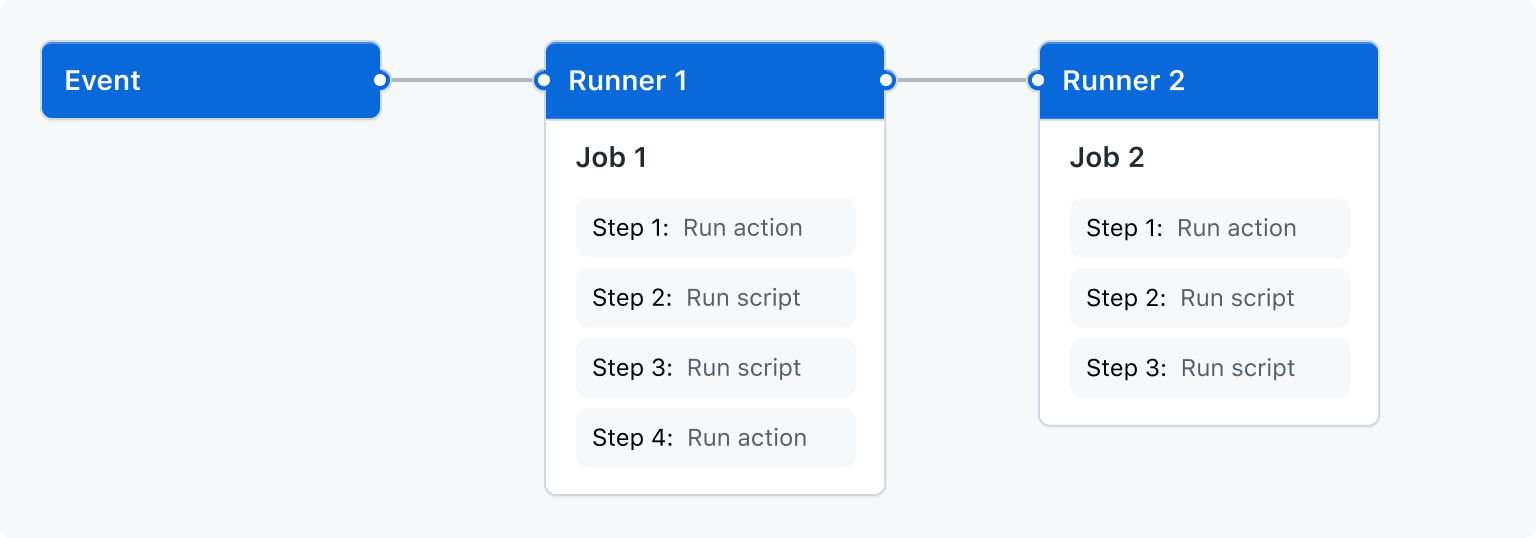
\includegraphics[width=130mm]{overview-github-actions.png}
  \caption[Components of GitHub Actions]{Components of GitHub Actions \cite{githubactions}}
  \label{github actions}
\end{figure}

\subsubsection{Workflows}
A workflow is a programmable automated procedure that executes one or more tasks. Workflows are specified in a YAML file that is checked into your repository. They can be triggered by an event in your repository, manually, or on a set timetable.

A repository can contain numerous workflows, each of which can carry out a separate set of tasks. For example, you may have one workflow to build and test pull requests, another to deploy your application whenever a release is made, and still another to add a label if someone reports a new issue.

\subsubsection{Events}
A workflow run is triggered by an event, which is a specific activity in a repository. For example, GitHub can be an activity when someone creates a pull request, opens an issue, or pushes a commit to a repository. A workflow can also be started manually on a timetable, or by triggering a REST API.

\subsubsection{Jobs}
A job is a series of workflow stages that all run on the same runner. Each step consists of either a shell script that will be run or an action that will be performed. The steps are carried out in a sequential order and are interdependent. Because each step is run on the same runner, data can be shared from one step to the next. A step that builds your application, for example, could be followed by a step that tests the application that was built.

You can configure a job's dependencies with other jobs; by default, jobs execute in parallel and have no dependencies. When a job becomes reliant on another job, it will not run until the dependent job has completed. You might have many build tasks for different architectures with no dependencies and a packaging job that is dependent on those jobs, for example. The build jobs will run in parallel, and the packaging job will begin once they have all completed successfully.

\subsubsection{Actions}
An action is a GitHub Actions platform custom application that performs a sophisticated but regularly repeated activity. To assist in limiting the amount of repetitive code in your workflow files, use an action. An action can grab your git repository from GitHub, configure your build environment's toolchain, or set up your cloud provider's credentials.

\subsubsection{Runners}
When your workflows are triggered, a runner is a server that executes them. Each runner is limited to one job at a time. To run your workflows, GitHub provides Ubuntu Linux, Microsoft Windows, and macOS runners; each workflow run takes place in a new, freshly provisioned virtual machine. You can host your own runners if you need a different operating system or a specific hardware setup.

\section{Library Implementation}
In this section, the implementation of the library is showcased and explained. The library will have 8 distinct project management objects each represented as a class in the library namely;

\begin{itemize}
  \item \verb +ProjectCharter+ class
  \item \verb +Stakeholder+ class
  \item \verb +Deliverable+ class
  \item \verb +ProjectGovernance+ class
  \item \verb +Risk+ class
  \item \verb +WBSItem+ class
  \item \verb +WBS+ class
  \item \verb +Project+ class
\end{itemize}

\subsection{The ProjectCharter class}
A project charter is a formal, typically short document that describes your project in its entirety — including what the objectives are, how it will be carried out, and who the stakeholders are. It is a crucial ingredient in planning the project because it is used throughout the project lifecycle \cite{wrike}.

The \verb+ProjectCharter+ class presents a few methods and properties.

The class's methods and signatures are represented below in a very simplified interface to abstract away the implementation.\\
\begin{lstlisting}
  class ProjectCharter(project_title = None):
      # properties
      property executive_summary: str
      property project_stakeholders: list
      property project_title: str

      # methods
      method add_stakeholder(self, stakeholder)

      # static methods
      static is_class_stakeholder(obj) -> bool
\end{lstlisting}

The constructor is called anytime a new \verb+ProjectCharter+ instance is created. It takes an optional argument, \verb+project_title+ and goes ahead to initialize an empty list \verb+_project_stakeholders+ private property that will hold and track \verb+Stakeholder+ objects

The \verb+executive_summary+ property is a string field that holds summarized information about project.

There's a restriction to the \verb+ProjectCharter+ class in that only objects initialized from the \verb+Stakeholder+ class can be added to the \verb+project_stakeholders+ list. \linebreak Adding a stakeholder must be done through the method \verb+add_stakeholder+. A static method \verb+is_class_stakeholder+ is available solely for verifying objects before they are accepted to the stakeholder list. The static method simple returns a boolean \verb+True+ or \verb+False+ and is used in the method \verb+add_stakeholder+ like below\\*

\begin{lstlisting}
  def add_stakeholder(self, stakeholder):
      assert self.is_class_stakeholder(stakeholder)
      if isinstance(stakeholder, (list, tuple)):
          for s in stakeholder:
              self.__finalize_add_stakeholder(s)
      else:
          self.__finalize_add_stakeholder(stakeholder)
\end{lstlisting}

\vfill

\begin{lstlisting}
  @staticmethod
  def is_class_stakeholder(obj) -> bool:
      """
      Checks that the stakeholder about to be added to the project
      is instance of the Stakeholder class
      """
      if isinstance(obj, list):
          return all(isinstance(s, Stakeholder) for s in obj)
      return isinstance(obj, Stakeholder)
\end{lstlisting}


\subsection{The Stakeholder class}
This class provides a template for modelling stakeholder objects. Its methods, properties and signatures are below in a simplified interface.

\begin{lstlisting}
  class Stakeholder(first_name, last_name, email):
      # methods
      method add_to_involved_projects(self, value)
      method get_full_name(self) -> str
      method get_number_of_projects(self) -> int

      # properties
      property projects_involved: List[Project]
      property responsibility: str
      property role
      property stakeholder_title
      property stakeholder_type
\end{lstlisting}

The method \verb+add_to_involved_projects+ is designed to be used only by the \linebreak \verb+__finalize_add_stakeholder()+ private method defined in the \verb+ProjectCharter+ class. It is simply used to add new \verb+ProjectCharter+ instances to the list of projects the stakeholder in question is involved with.

\verb+get_number_of_projects()+ simply returns an integer depicting the number of projects that stakeholder instance is involved with at any point in time.

The property \verb+projects_involved+ returns a list of objects of the \verb+ProjectCharter+ charter class readily available should the library consumer require it.

For the \verb+role+ property of the various stakeholders, a simple enum following the RACI responsibility models is defined.

\begin{lstlisting}
  class RoleEnum(Enum):
      """
      * R = Responsible (Those who do the work to complete the task)
      * A = Accountable (also approver or final approving authority)
      * C = Consulted (Those whose opinions are sought)
      * I = Informed (Those who are kept up-to-date on progress)
      """

      RESPONSIBLE = "R"
      ACCOUNTABLE = "A"
      CONSULTED = "C"
      INFORMED = "I"
      UNSET = "UNSET"
\end{lstlisting}


\subsection{The Deliverable class}
Deliverables are very important to the success of any project and this library provides an implementation of a deliverable model. The methods and properties it provides are showcased in the simple interface below

\begin{lstlisting}
  class Deliverable(doc_title):
      # methods
      method mark_as_accepted(self)
      method mark_as_rejected(self)
      method set_reviewer(self, value)

      # properties
      property accepted: bool
      property reviewer
      property acceptance_criteria
      property description
      property expected_result
\end{lstlisting}

The \verb+mark_as_accepted+ and \verb+mark_as_rejected+ methods serve to set the \verb+accepted+ property to \verb+True+ or \verb+False+ depending on whether the deliverable has been accepted or not. \verb+set_reviewer+ sets the \verb+reviewer+ property to the "responsible" who is accountable for the deliverable. \verb+acceptance_criteria+ property serves to define what determines when a deliverable can be accepted or not.


\subsection{The ProjectGovernance class}
Project Governance is the set of rules, procedures and policies that determine how projects are managed and overseen.

These rules and procedures define how decisions are made during projects. As part of the oversight process, project governance also determines the metrics by which project success is measured.

The methods and properties this class implements are in the simplified interface below.

\begin{lstlisting}
  class ProjectGovernance(project):
      # methods
      method get_all_stakeholders(self) -> list
      method sign_agreement(self, signee: Stakeholder)

      # properties
      property not_signed_by: list
      property signed_by: list
      property signed_by_all: bool
\end{lstlisting}

The \verb+get_all_stakeholders+ method simply returns a list of stakeholder objects included in the current project governance object.

\verb+sign_agreement+ simply exposes a method used to sign the project governance by the stakeholder object passed in the argument.

There are a few properties in this class as well. \verb+not_signed_by+ returns a list of stakeholder objects included in the project governance object but has yet to consent the terms that will govern the project execution. \verb+signed_by+ also returns a list of stakeholder objects and is the exact opposite of the former.
\verb+signed_by_all+ is a boolean type that simple returns \verb+True+ if all the involved stakeholders have signed and \verb+False+ otherwise.


\subsection{The Risk class}
Risk is any unexpected event that can affect your project — for better or for worse \cite{wrike-2}. People, processes, technology, and resources can all be impacted by risk. Risks are not the same as issues, which is a crucial distinction to recognize. Issues are something you know you'll have to deal with and may even know when they'll happen, such as a planned vacation for a team member or a large rise in product demand during the holidays. Risks are occurrences that can happen at any time and that you may not be able to predict — for example, a sudden outbreak of flu in your office or a critical product component being out of stock.

The \verb+Risk+ class for this library has an interface as showcased below

\begin{lstlisting}
  class Risk(risk_name, probability, impact)
      # methods
      method assign_risk_owner(self, value)
      method get_risk_score(self)
      method set_counter_measure(self, counter_measure)

      # properties
      property counter_measure
      property description
      property impact
      property probability
      property risk_owner
\end{lstlisting}

\verb+assign_risk_owner+ is simply the method for assigning the risk owner. \linebreak \verb+get_risk_score+ is a value calculated based on the \verb+probability+ and \verb+impact+ \linebreak properties. An Enum class \verb+RiskScore+ is defined to organize the various risk score points and is the return type of the method \verb+get_risk_score+.

\begin{lstlisting}
  class RiskScore(Enum):
      VERY_HIGH = range(80, 101)  # 80% - 100%
      HIGH = range(50, 80)  # 50% - 79%
      MODERATE = range(30, 50)  # 30% - 49%
      LOW = range(0, 30)  # 0 - 29%

      @classmethod
      def get_risk_score(cls, value):
          for val in cls:
              if value in val.value:
                  return val
\end{lstlisting}

The \verb+set_counter_measure+ method is responsible for setting the counter measure to be adopted for mitigating the particular risk object in question.

There are a possible of allowed values for the return value of the \verb+set_counter_measure+ method. It is defined in the \verb+RiskCounterMeasure+ Enum class

\begin{lstlisting}
  class RiskCounterMeasure(Enum):
      REDUCE = "REDUCE"
      PREVENT = "PREVENT"
      ACCEPT = "ACCEPT"
      TRANSFER = "TRANSFER"

      @classmethod
      def list_allowed_values(cls):
          return list(map(lambda c: c.value, cls))
\end{lstlisting}


\subsection{The WBS class}
The \ac{wbs} class provides an interface for organizing objects from the \verb+WBSItem+ class. The \verb+WBSItem+ class's properties are displayed below

\begin{lstlisting}
  class WBSItem(work_item_name, duration, lag):
      # properties
      property duration
      property lag
      property objective
      property percent_complete
      property resource
      property status
\end{lstlisting}

Several \verb+WBSItem+ objects are aggregated under a list type property to make up part of the \verb+WBS+ class.

Here is a look at the \verb+WBS+ class simplified interface

\begin{lstlisting}
  class WBS(name, start_date):
      # methods
      method add_wbs_item(self, *args: WBSItem)
      method get_critical_path(self)
      method link_nodes(self, *args: Tuple[WBSItem, WBSItem])
      method update_all(self)

      # properties
      property duration
      property finish_date
      property percent_complete
      property start_date
      property wbs_items: List[WBSItem]
\end{lstlisting}

The method \verb+add_wbs_item+ takes as many arguments as are passed to it which themselves must be objects made from the \verb+WBSItem+'s class. The method adds the individual \verb+WBSItem+ objects to the \verb+WBS+ object into the property \verb+wbs_items+

It is important to mention that the \verb+WBS+ class makes use of an external python package (library), \verb+criticalpath+ \cite{criticalpath}. It uses the CPM method to calculate the critical path of a network of tasks, assuming the graph in question is acyclic (i.e. has no closed loops)

The method \verb+get_critical_path+ calculates the critical path of the graph utilizing the \verb+criticalpath+ package. The method returns a visual string representation of the critical path of the graph in question.

\verb+link_nodes+ takes as many tuple type arguments of \verb+WBSItem+ objects to link to one another

An example usage from a test case is shown below. \linebreak

\begin{lstlisting}
  def test_WBS_link_nodes(wbs: WBS, wbs_item_factory):

      ...

      node_pairs = (
          (node1, node2),
          (node2, node3),
          (node3, node6),
          (node6, node7),
          (node2, node4),
          (node4, node6),
          (node2, node5),
          (node4, node5),
          (node5, node7),
      )
      wbs.link_nodes(*node_pairs)
      wbs.duration.days  # 29
      wbs.get_critical_path() # "node1 -> node2 -> node4 -> node6 -> node7"
\end{lstlisting}

The graph that produced the \verb+node_pairs+ in the example above will look like in the image in \autoref{node pairs}.

\begin{figure}[H]
  \centering
  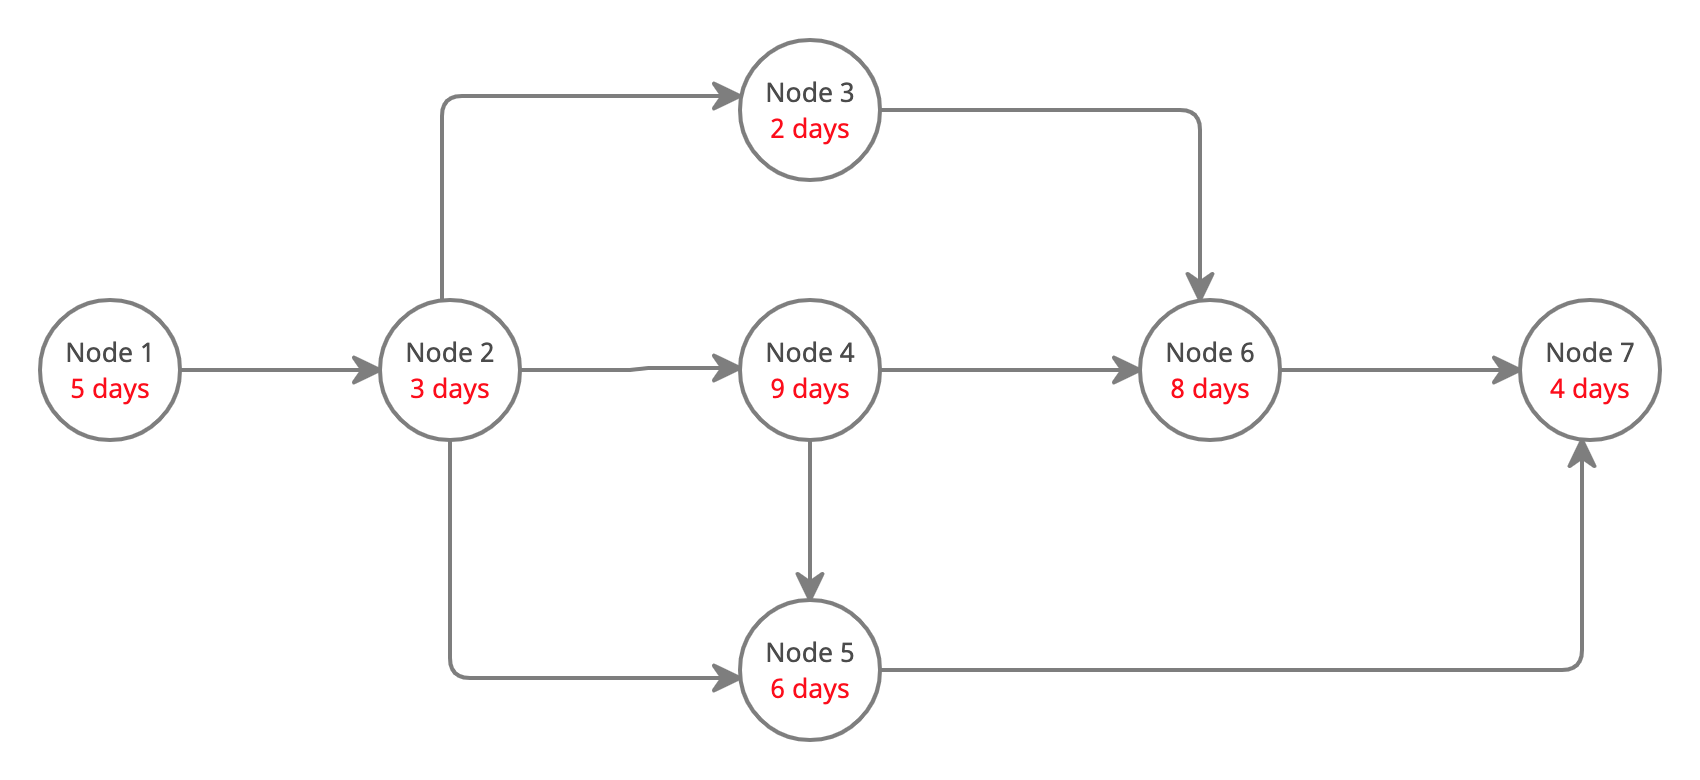
\includegraphics[width=130mm]{activity_graph.png}
  \caption{Sample activity node diagram}
  \label{node pairs}
\end{figure}

Each node pair has to be represented in order to ensure accurate results when accessing the \verb+.duration.days+ property or even while calling the \linebreak\verb+.get_critical_path()+. Repitions are ignored. For \autoref{node pairs}, the relevant node pairs are 

\begin{itemize}
  \item node1, node2
  \item node2, node3
  \item node3, node6
  \item node6, node7
  \item node2, node4
  \item node4, node6
  \item node2, node5
  \item node4, node5
  \item node5, node7
\end{itemize}


\subsection{The Project class}
The project class serves as a demonstration as to how the other class objects can be managed under a common umbrella. It provides an interface for interacting with other objects and performing operations on them.

\begin{lstlisting}
  class Project(project_charter):
      # methods
      method create_deliverable(self, deliverable_name)
      method add_deliverable(self, deliverable: Deliverable)
      method accept_deliverable(self, deliverable: Deliverable)
      method reject_deliverable(self, deliverable: Deliverable)
      method add_new_project_risk(self, risk)

      # properties
      property deliverables
      property project_risks
      property project_charter
      property stakeholders
      property project_governance
\end{lstlisting}

\verb+.create_deliverable()+ method take an argument, \verb+deliverable_name+ and returns an object of type \verb+Deliverable+. It also calls the method \verb+.add_deliverable()+ with the newly created \verb+Deliverable+ object as the only argument.

\verb+.accept_deliverable()+ and \verb+.reject_deliverable()+ are light wrappers around the Deliverable objects and serve to mark the deliverable objects as accepted or rejected using the methods \verb+.mark_as_accepted()+ and \verb+.mark_as_rejected()+ which the deliverable objects provides themselves.

\begin{lstlisting}
  class Project:

      ...

      def accept_deliverable(self, deliverable: Deliverable):
          assert deliverable in self._deliverables, "Deliverable does not exist within the current project"
          deliverable.mark_as_accepted()

      def reject_deliverable(self, deliverable: Deliverable):
          assert deliverable in self._deliverables, "Deliverable does not exist within the current project"
          deliverable.mark_as_rejected()
\end{lstlisting}


\section{Testing}
